\documentclass[11pt,a4paper]{ctexart}
\usepackage{geometry}
\geometry{margin=2cm}
\usepackage{graphicx}
\usepackage{xcolor}
\usepackage{tcolorbox}
\usepackage{booktabs}
\usepackage{tabularx}
\usepackage{array}
\usepackage{tikz}
\usepackage{enumitem}
\usepackage{microtype}
\usepackage{titlesec}
\usepackage{float}
\usepackage{caption}
\usepackage{hyperref}
\usetikzlibrary{shapes.geometric,arrows.meta,positioning,fit,backgrounds}

\definecolor{primary}{RGB}{230,150,0}
\definecolor{ink}{RGB}{40,40,40}
\definecolor{soft}{RGB}{120,120,120}
\hypersetup{colorlinks=true,linkcolor=primary,urlcolor=primary}
\captionsetup{font=small,labelfont={bf,color=primary}}

\titleformat{\section}[block]
  {\Large\bfseries\color{primary}}
  {\thesection}{0.6em}{}
  [\vspace{-0.3em}{\color{primary}\rule{\linewidth}{1pt}}]
\titleformat{\subsection}[block]
  {\large\bfseries\color{ink}}
  {\thesubsection}{0.5em}{}

\newtcolorbox{keybox}[1]{colback=primary!7,colframe=primary!55,title=#1,fonttitle=\bfseries,left=3pt,right=3pt,top=3pt,bottom=3pt}

% 一张大图
\newcommand{\shot}[3]{%
\begin{figure}[H]\centering
\includegraphics[width=#3\linewidth]{assets/#1}
\caption{#2}
\end{figure}}

\begin{document}

% ---------------- 封面 ----------------
\begin{titlepage}
  \centering
  \vspace*{2.2cm}
  {\Huge\bfseries\color{primary} 小悠 · YOYU}\\[0.5cm]
  {\LARGE 一个会陪你过周末的 AI 本地生活浏览器}\\[1.1cm]
  {\large 跑在你自己电脑上，带着你的登录态去真读点评/必吃榜/小红书/高德，}\\[0.15cm]
  {\large 帮你把"周末这几个小时"安排明白；越用越懂你、会主动惦记你，}\\[0.15cm]
  {\large 数据还留在你自己电脑里。}\\[1.8cm]
  {\normalsize 美团黑客松 · 赛题 06「本地探索：周末闲时活动规划」}\\[0.5cm]
  {\normalsize 方案设计文档（给导师看的版本）}\\[1.6cm]
  {\small 代码仓库：\url{https://github.com/bcefghj/YOYU}}\\[0.3cm]
  {\small 2026 年 7 月}
  \vfill
\end{titlepage}

\tableofcontents
\newpage

% ---------------- 一句话 ----------------
\section{一句话：小悠是干嘛的}

\begin{keybox}{给导师的大白话}
临时想"这周末带娃/陪老婆/陪爸妈出去转转"，但不知道去哪、懒得挨个查、约人又费劲、到店还怕踩雷。\textbf{小悠就是帮你把这件事一句话搞定}：它是一个装在你电脑上的浏览器，你说一句"周六下午带孩子出去玩4小时、老婆减脂、人均120"，它就自己去点评/高德把真店、真路线、真评价查出来，一次给你三套方案，还能帮你点菜、排号、发家人确认。用得越多它越懂你，到周末还会主动问你要不要安排。
\end{keybox}

我们不重做美团，美团已经很好了。我们做的是\textbf{站在美团这些平台之上、帮用户把它们用得更顺的一层}。下面全是真机截图，导师您看图就知道我们在做什么。

\shot{01_current.png}{小悠主界面：左边工具栏，中间是内置浏览器（带美团/点评/高德/小红书收藏夹），右边是小悠对话。右上角黄色卡片是它"主动想起你"——记得你喜欢的店，问你这周要不要再约一次。}{0.96}

% ---------------- 核心功能（配图） ----------------
\section{核心功能（一个个看图）}

\subsection{1. 一句话，出三套真实方案}
你说一句话，它自动定位你在的城市（这里是深圳），一次给\textbf{经济/均衡/特色}三套方案，每套都有真实店铺、真实人均、真实评分，配一张真高德地图画出路线，还有一个五维雷达图（省钱/好玩/便捷/合适/特色）。右边"执行过程"是透明的，能看到它在并行找玩乐和餐厅、去水分、组装时间线、还自己校验有没有超预算。

\shot{08_steps.png}{三套方案 + 真实地图路线（2.2km/10分钟）+ 五维雷达。右侧透明展示"多 Agent 在干活"。}{0.96}

\shot{09_result.png}{方案给完后，小悠用大白话补一段解释：数据来源真实、还给了两套备选、以及"你接下来可以做什么"（比价/点菜/发老婆确认/一键排号）。}{0.96}

\subsection{2. 它是真的会自己开网页、看网页（AI 操控浏览器）}
这是我们最想给导师看的一点：小悠\textbf{真的能自己打开大众点评、看懂页面}。下图里它读取了深圳大众点评首页，用彩色编号框把页面上所有"能点的地方"都标了出来（这叫 Set-of-Marks），右边同步显示"读取当前页·真实"。这不是截图拼的，是它自己开的真页面。

\shot{14_som.png}{AI 操控浏览器：小悠打开真实的深圳大众点评，把页面上可点的元素全部用彩色编号框标出来，再逐个读取内容。按钮绿、链接蓝、输入框紫。}{0.96}

\shot{10_browser_dianping.png}{内置浏览器打开的真实大众点评深圳站（登录后就能读到你自己的收藏、券、排队号）。}{0.96}

\subsection{3. 越用越懂你 + 数据留在你电脑里}
小悠会把你的口味、常带的人、常去的店慢慢记下来，下次规划自动带上。下图是它的"记忆"：陪你多少天、一起去过几个地方、你的偏好（老婆减脂 $\times$6 次、常带 5 岁女儿、偏爱杭帮菜/粤菜、不爱排队超 30 分钟）、常去的店、还有周末足迹时间线。\textbf{最上面绿色那条最重要：这些记忆只存在你这台电脑，不上传服务器，可查、可删。}

\shot{04_memory.png}{"小悠记住的你"：偏好带出现次数、常去店、周末足迹。顶部绿条=数据留本机、可删。这就是"越用越懂你"和"数据主权"。}{0.7}

\subsection{4. 点菜：招牌菜推荐 + 按人群避雷}
以海底捞为例：它给出招牌/热销菜，同时按你家情况列出"建议避开的"——麻辣锅底（老婆减脂大忌）、油炸响铃（热量炸弹）、甜品（孩子/减脂少吃），每条都给了原因，还顺手教你把芝麻酱换成小米辣蘸料。

\shot{13_dishes.png}{AI 点菜：左边招牌菜，右边"建议避开的"带原因，全部按"老婆减脂+5岁孩子"来定制。}{0.96}

\subsection{5. 排队取号（半自动，最后一步你确认）}
海底捞这种要排队的店，小悠能帮你线上取号，把号码、前面几桌、预计多久都拿回来，到点提醒你出发。注意它\textbf{诚实标了"模拟"}，因为真实取号需要登录，演示阶段先模拟。

\shot{15_queue.png}{排队取号：拿到 A67 号、前面 5 桌、约 35 分钟，建议先去逛、到点提醒。诚实标注"模拟"。}{0.96}

\subsection{6. 点外卖、送花（都两步确认，绝不乱下单）}
不光到店，顺手的事它也能干：点份减脂外卖送到公司、给老婆订束花。所有\textbf{花钱的动作都要你再点一次"确认"}才真执行，安全。

\shot{16_takeout.png}{点外卖：按"减脂"配好轻食、能改送到家/公司、明细清楚，最后一步"确认下单"。}{0.96}

\shot{17_gift.png}{送花：生成"两步确认"卡——送到家、周六15:00、预算200，你不点"确认执行"它就不会真下单。}{0.96}

\subsection{7. 没想法时：附近发现 / 优惠发现}
不知道去哪的时候，点"附近发现"就弹出附近真实的美食和玩乐；点"优惠发现"看券后到手价，还会\textbf{识别假低价}。

\shot{02_discover.png}{附近发现：独立窗口弹出附近真实美食/玩乐，带图、评分、人均，可直接去规划或看路线。}{0.9}

\shot{03_deals.png}{优惠发现：按"券后省得多"排序，原价→到手价一目了然，标注"已识别假低价"。}{0.9}

\subsection{8. 方案发给家人：扫码就能看，还能投票}
生成的方案能\textbf{生成二维码}，家人同一个 WiFi 扫一下就能看方案、投票、留想法，你这边收到反馈再并入方案。

\shot{12_share.png}{发同行人确认：二维码 + 局域网链接，家人扫码看方案并投票（可以/一般/不行）。}{0.9}

\subsection{9. 页内路线：不跳出去，直接看怎么走}
点"路线"直接在应用里画出真实路线，驾车/地铁/步行都有距离和时间，只有真要打车时才跳高德。

\shot{11_route.png}{页内路线面板：真实地图 + 路线，7.9km/19分钟，驾车/公交地铁/步行随便切。}{0.9}

\subsection{10. 平台化：模型可换、技能可加、微信 24h 陪你}
\begin{itemize}[leftmargin=1.3em,itemsep=1pt]
  \item \textbf{模型可切换}：默认美团 LongCat，也能一键换 MiniMax/DeepSeek/Kimi。
  \item \textbf{技能可加装}：像装插件一样加能力（减脂友好、陪长辈、亲子遛娃、约会送花、纪念日惊喜……命中场景自动展开）。
  \item \textbf{微信 24h 陪伴}：连上微信后，人不在电脑前，到饭点/周末/纪念日它也会在微信里主动惦记你。
\end{itemize}

\begin{figure}[H]\centering
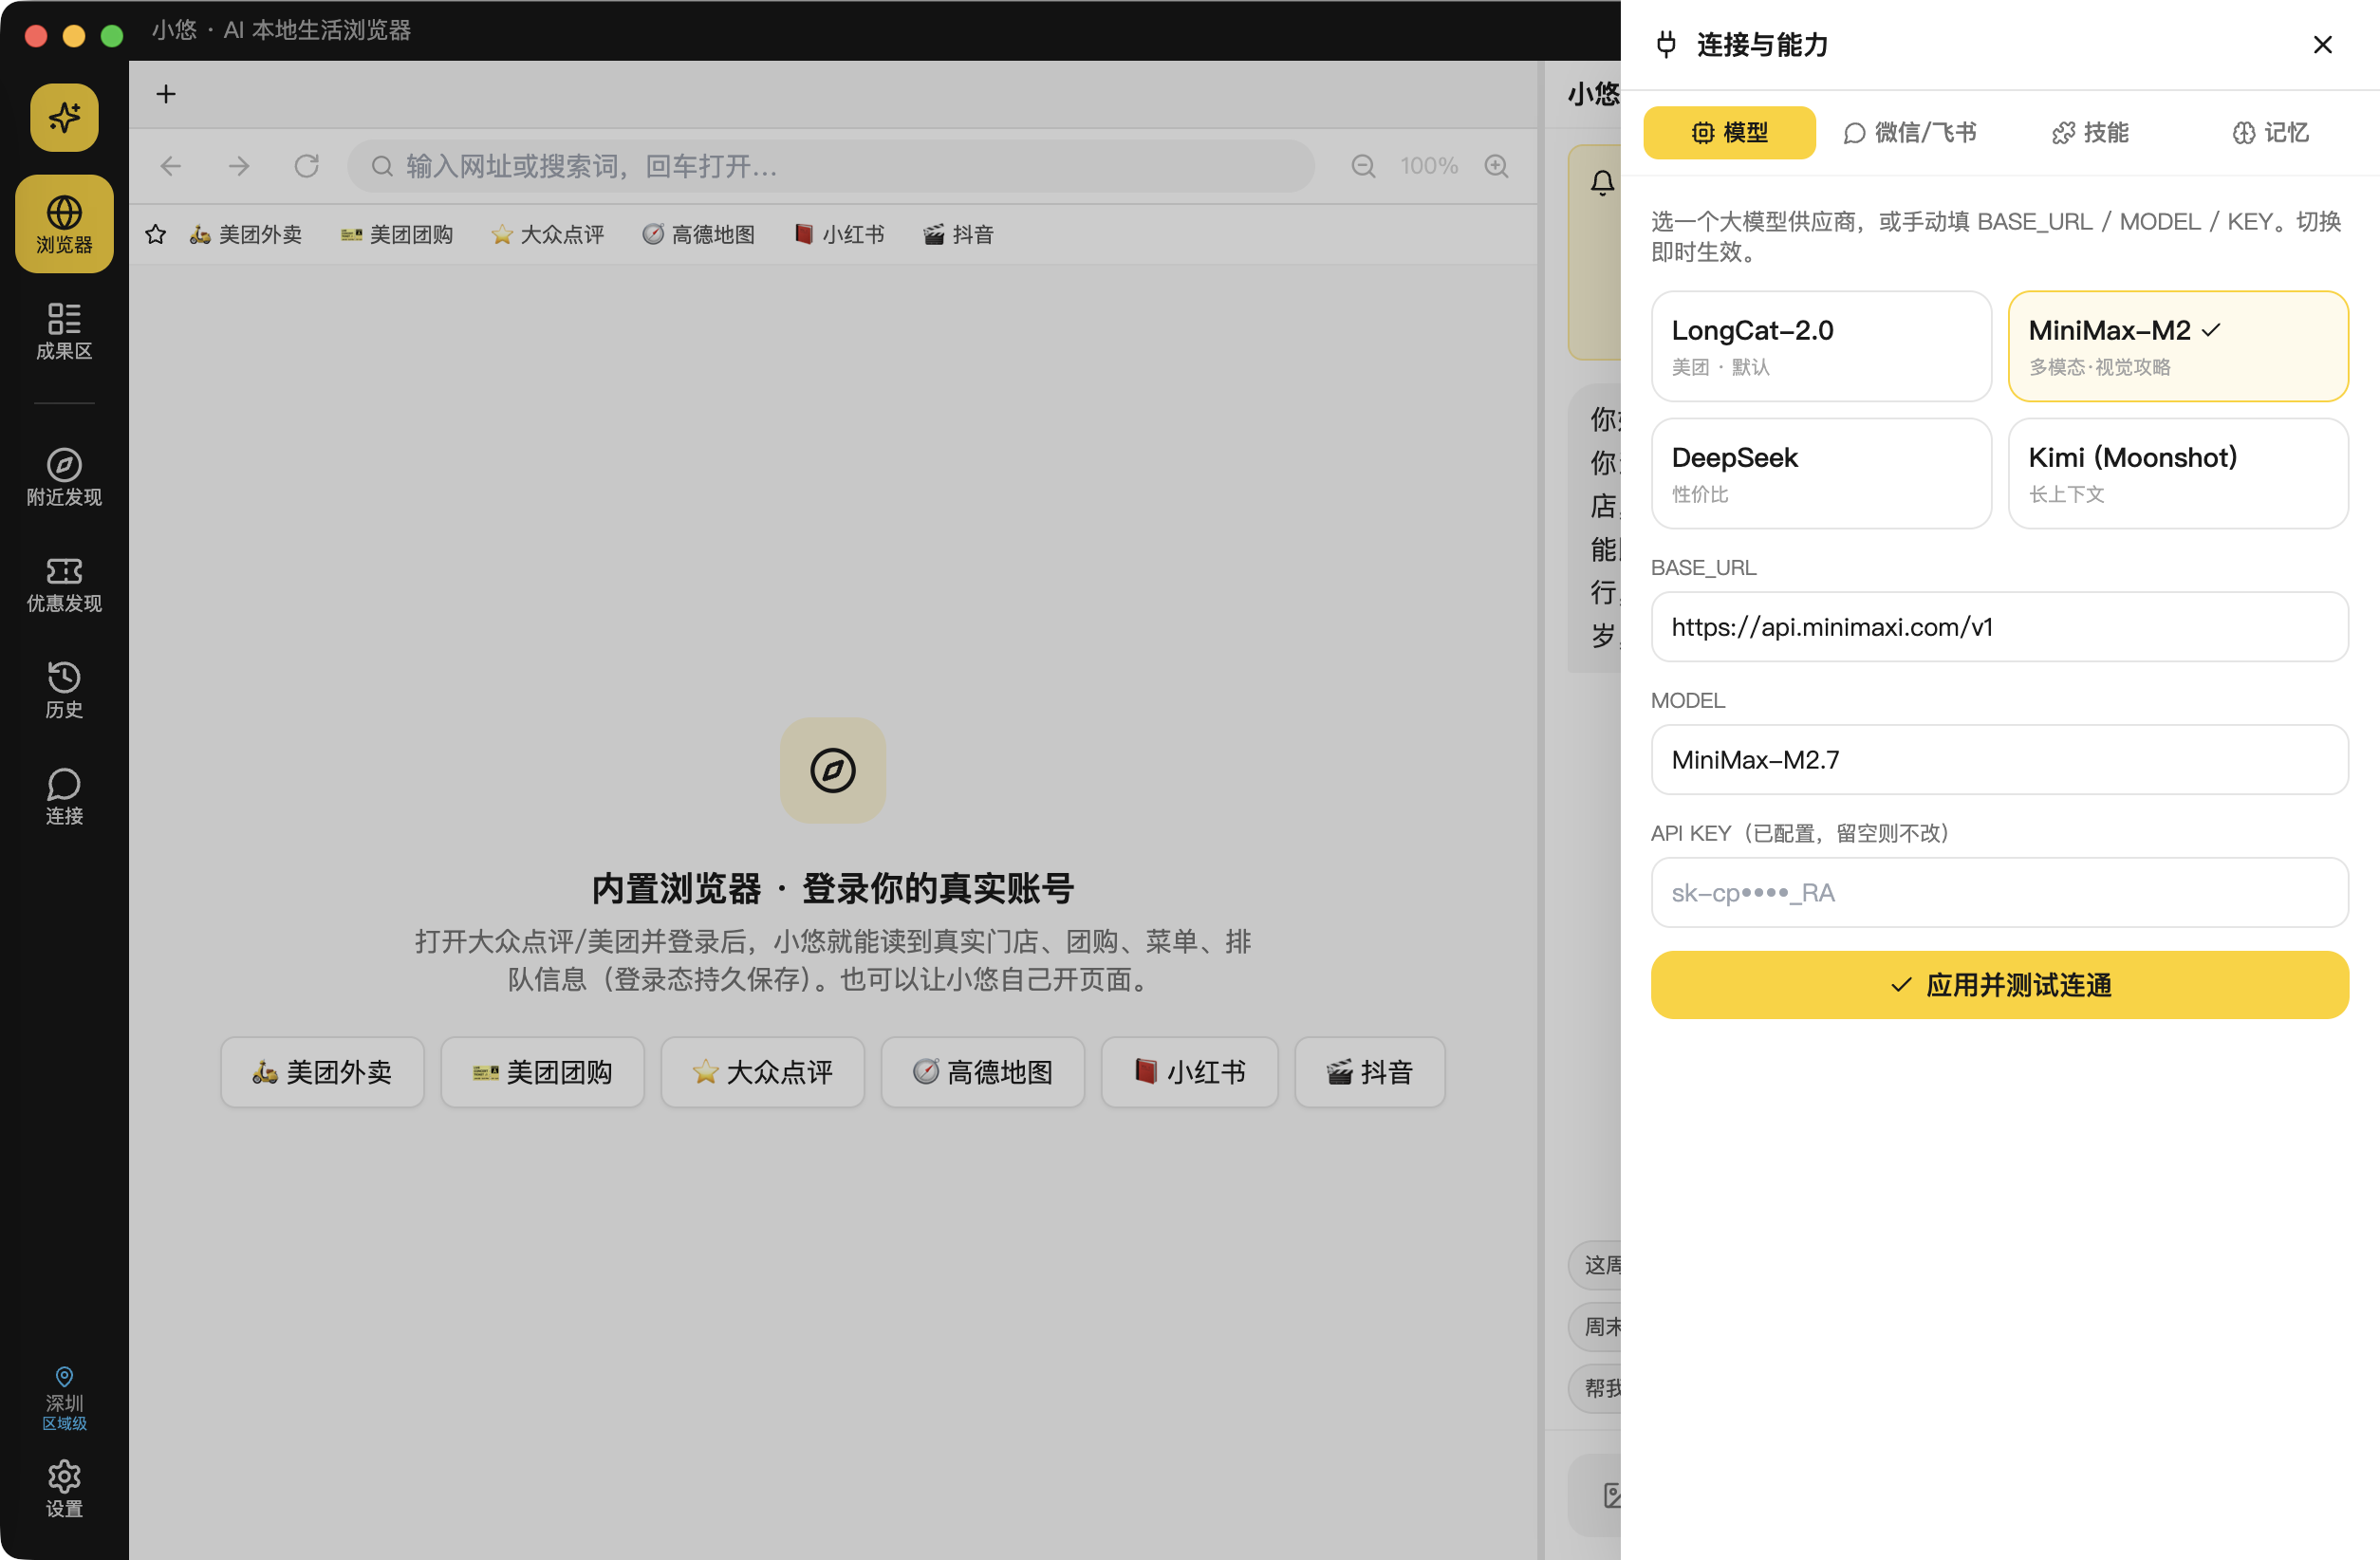
\includegraphics[width=0.32\linewidth]{assets/07_model.png}\hfill
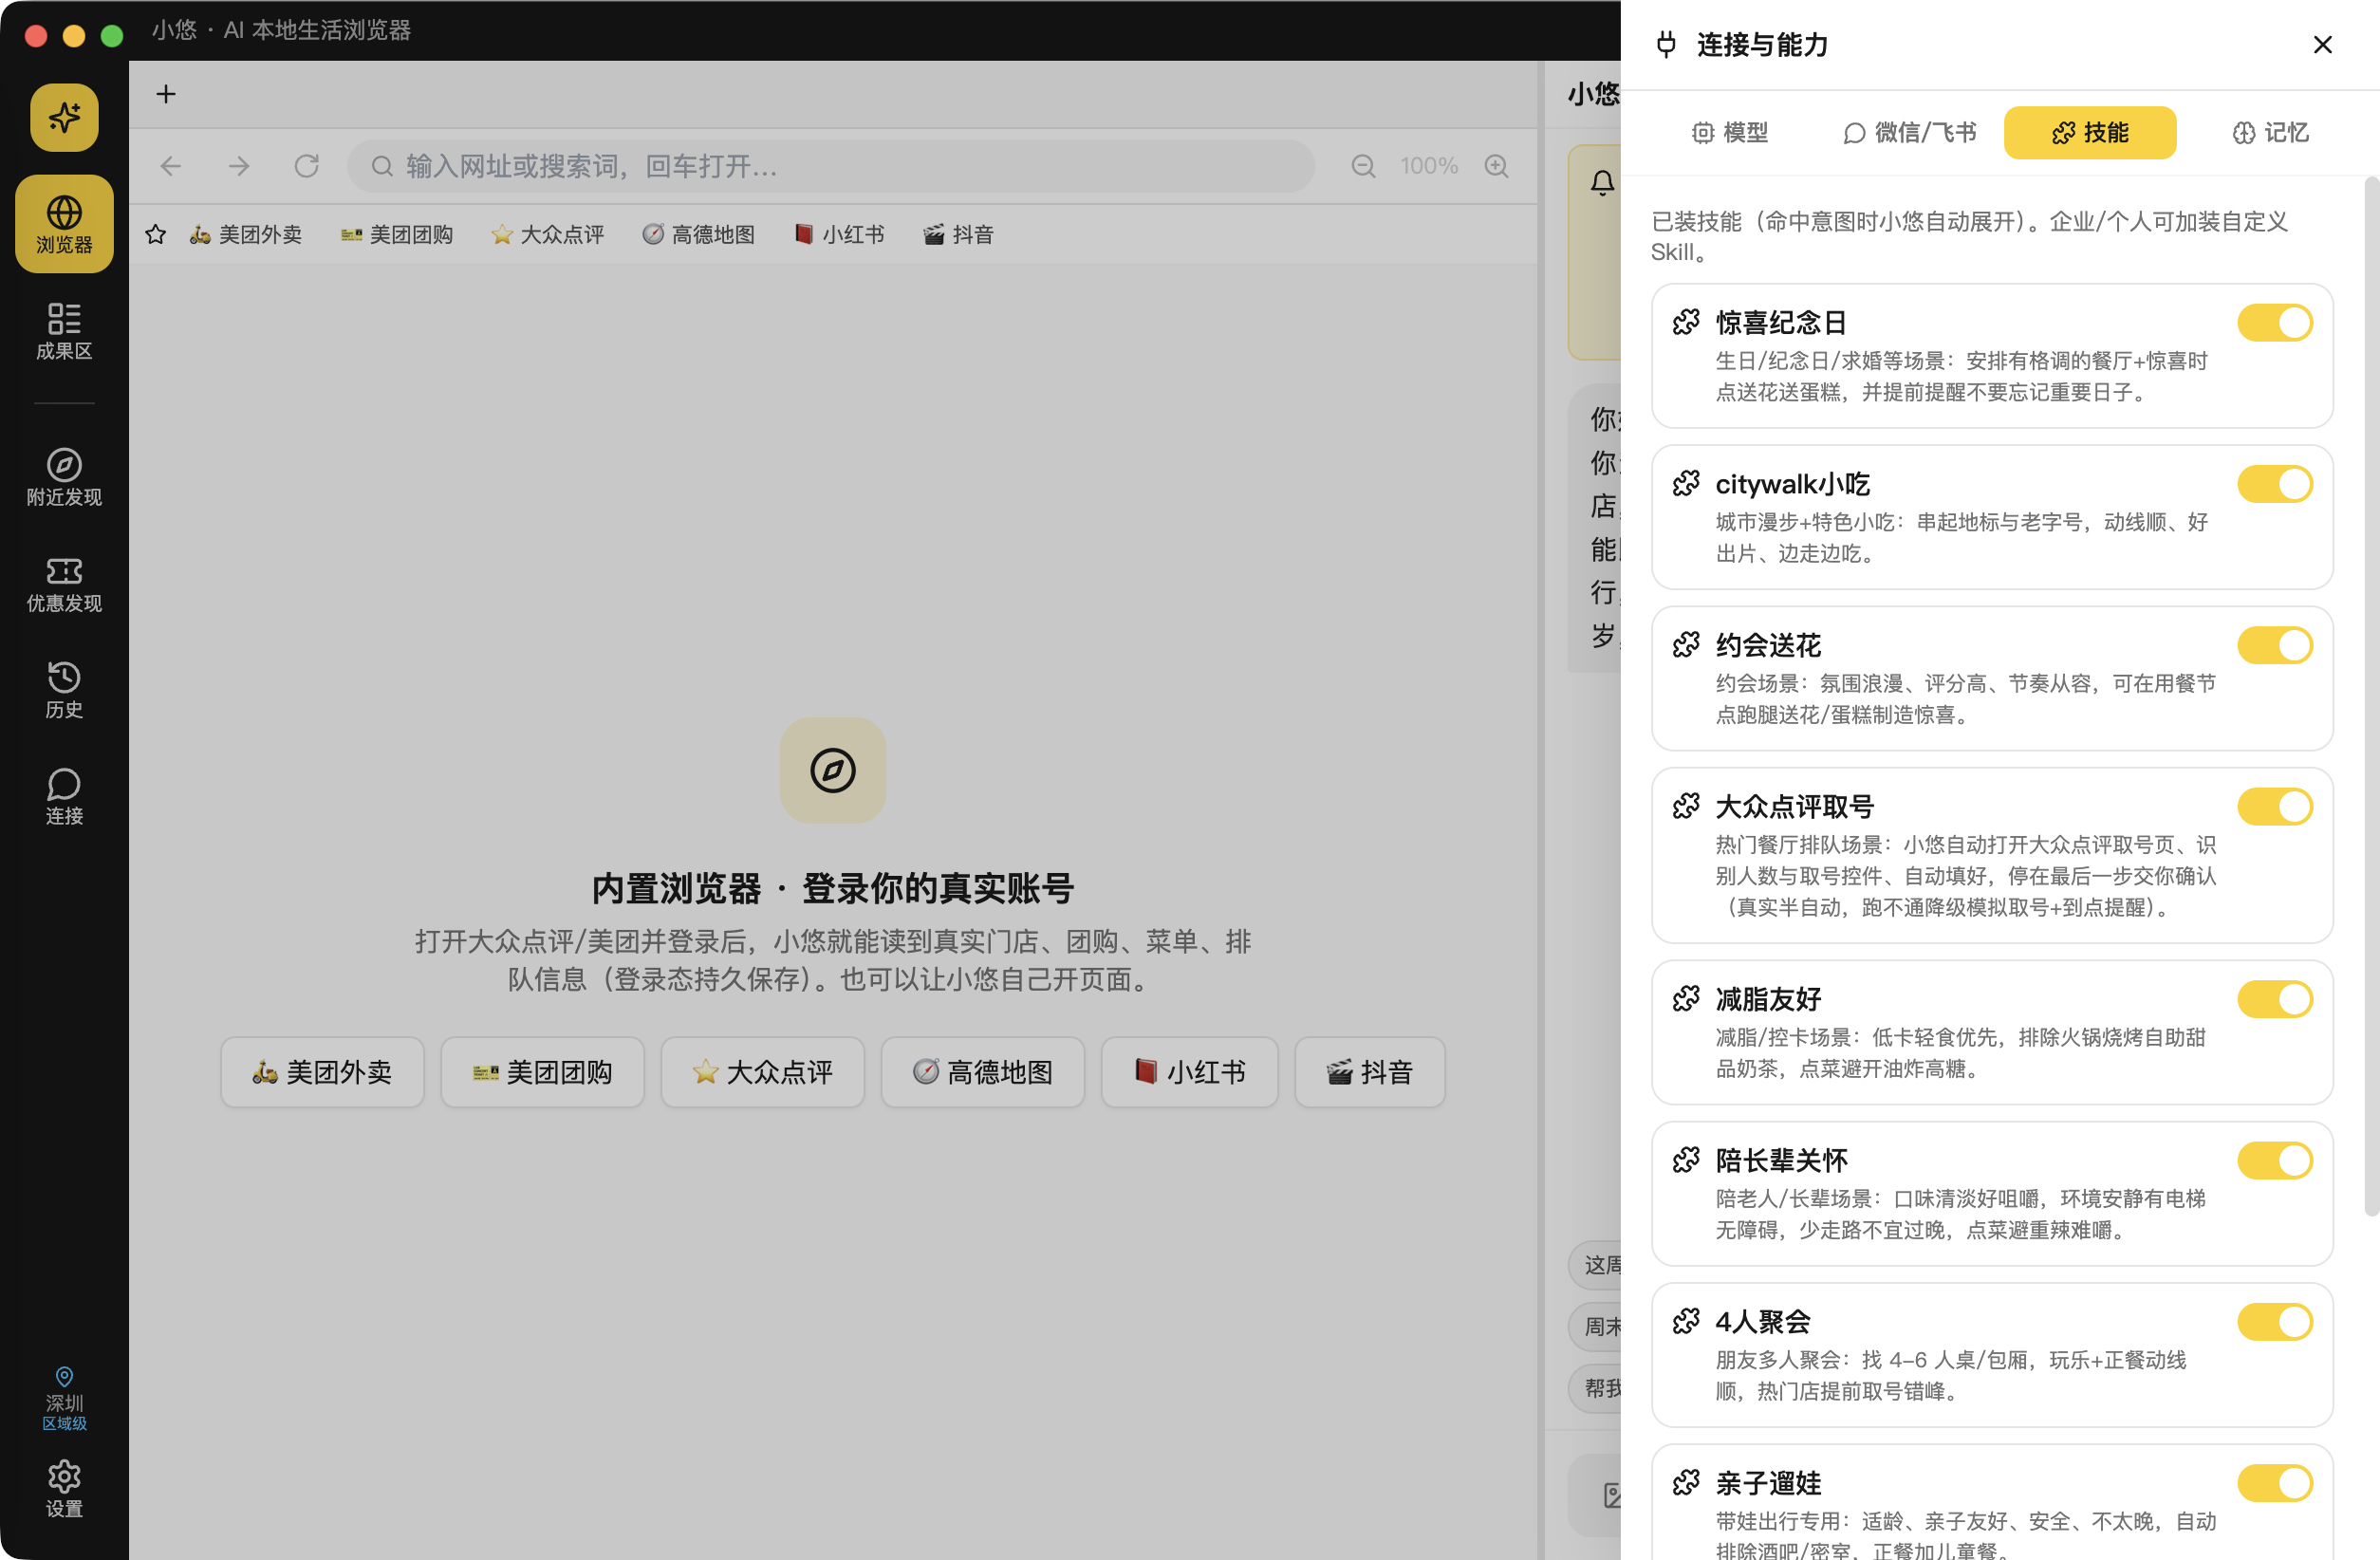
\includegraphics[width=0.32\linewidth]{assets/05_skills.png}\hfill
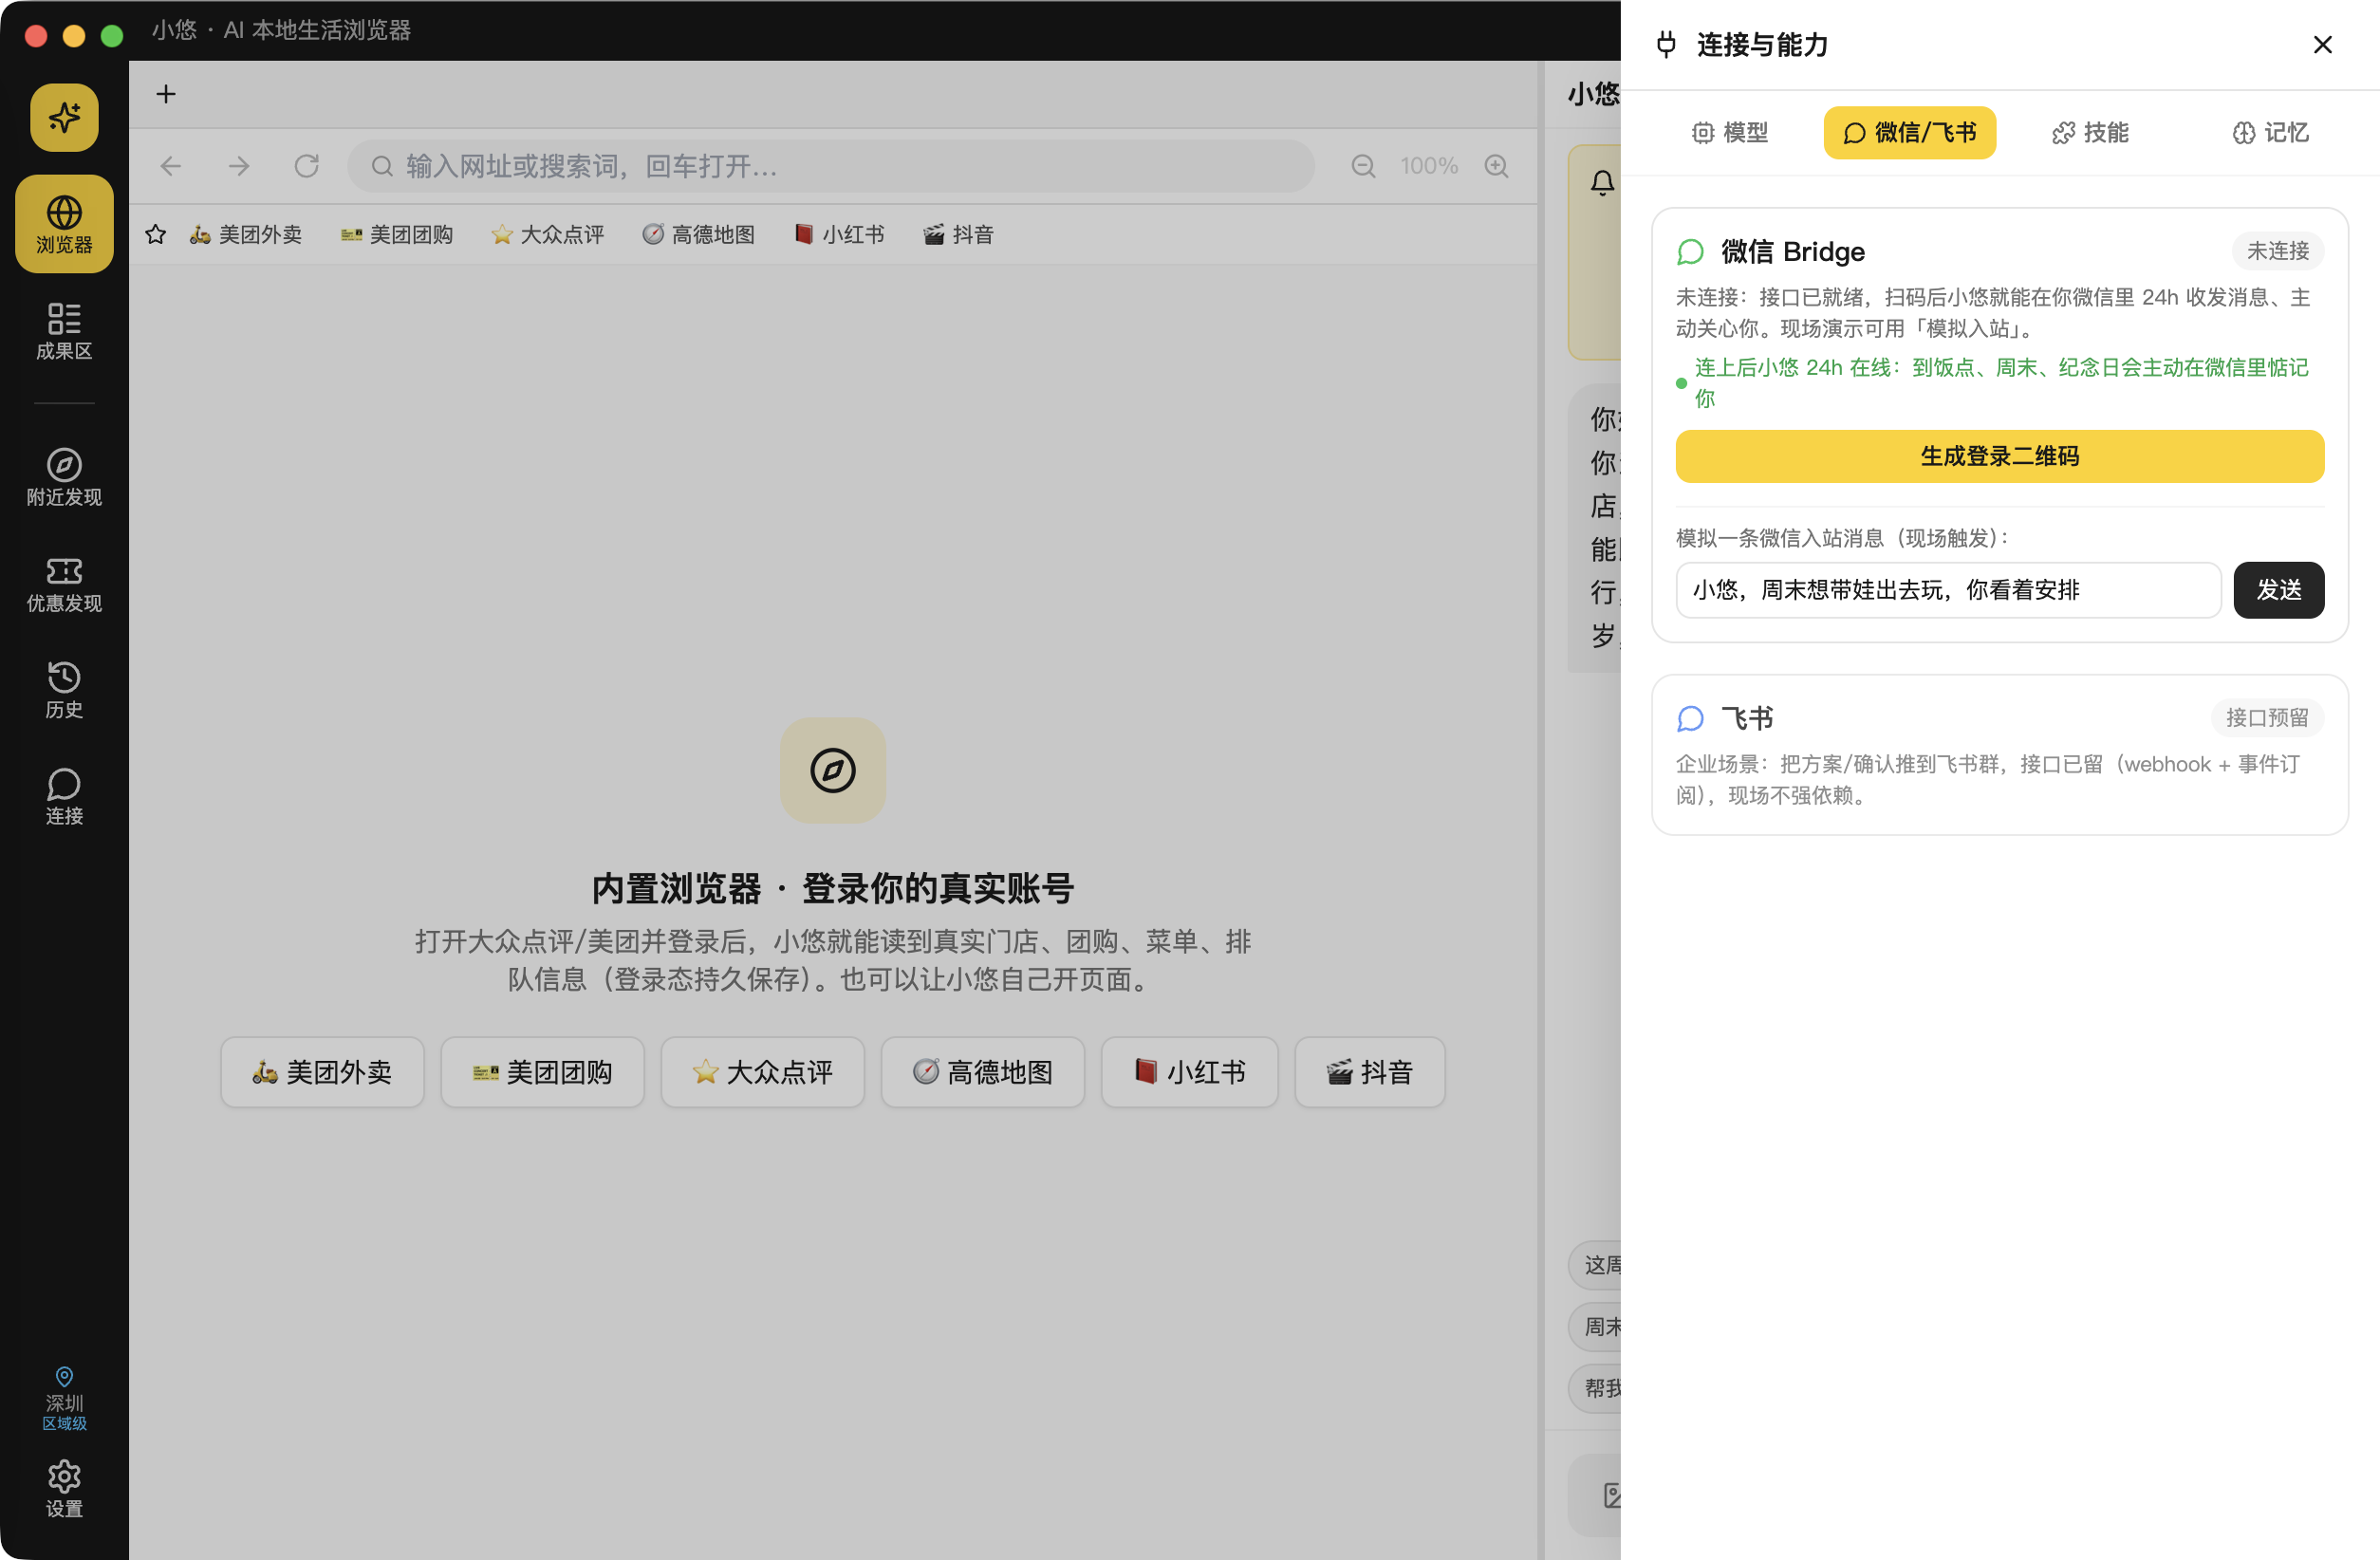
\includegraphics[width=0.32\linewidth]{assets/06_social.png}
\caption{左：换模型；中：技能面板（可开关/可加装）；右：微信 Bridge（连上后 24h 主动关心）。}
\end{figure}

\subsection{11. 聊天记录都留着}
每次对话和成果都存在左上角"历史会话"，随时翻回来。下图是一个用了一阵子的用户的记录。

\shot{18_history.png}{历史会话：过往的规划、点菜、取号、外卖都能翻回来。}{0.62}

% ---------------- 技术 ----------------
\section{技术上是怎么搭的}

\subsection{整体架构（五层）}
\begin{center}
\begin{tikzpicture}[
  layer/.style={draw, rounded corners=3pt, minimum width=13cm, minimum height=0.85cm, align=center, font=\small},
  arr/.style={-Latex, thick, color=primary},
]
\node[layer, fill=primary!16] (ui) {界面层：内置浏览器 + 成果区画布 + 对话 + 连接面板（Electron / React）};
\node[layer, fill=primary!11, below=0.4cm of ui] (agent) {Agent 层：主 Agent 派单 $\rightarrow$ 餐饮 / 玩乐 / 调研 / 记忆 子 Agent（多 Agent 协同）};
\node[layer, fill=primary!8, below=0.4cm of agent] (tool) {工具层：规划 / 点菜 / 比价 / 团购 / 外卖 / 取号 / 浏览器感知-动作 / 分享};
\node[layer, fill=primary!6, below=0.4cm of tool] (data) {数据层（可热插拔）：高德实时 / 本地数据集兜底 / 企业自有 API};
\node[layer, fill=primary!5, below=0.4cm of data] (mem) {记忆与陪伴：三层记忆（存本机）+ 主动关心 + 微信 Bridge};
\draw[arr] (ui) -- (agent);
\draw[arr] (agent) -- (tool);
\draw[arr] (tool) -- (data);
\draw[arr] (agent.east) to[bend left=42] (mem.east);
\end{tikzpicture}
\end{center}

\subsection{多 Agent 是怎么配合的}
主 Agent（小悠本体）像个组长，遇到复杂活就派给专家子 Agent，每个子 Agent 只拿自己该用的工具、独立干、只回结论。这个过程在界面右侧"执行过程"里是看得见的（对标美团 WOWService 的思路）。

\begin{center}
\begin{tikzpicture}[
  node distance=0.5cm and 0.9cm, font=\small,
  main/.style={draw, rounded corners=3pt, fill=primary!16, minimum width=2.6cm, minimum height=0.9cm, align=center},
  sub/.style={draw, rounded corners=3pt, fill=primary!8, minimum width=2.5cm, minimum height=0.8cm, align=center},
  arr/.style={-Latex, thick, color=primary},
]
\node[main] (m) {主 Agent · 小悠};
\node[sub, below left=1cm and 1.6cm of m] (a) {餐饮专家};
\node[sub, right=0.5cm of a] (b) {玩乐专家};
\node[sub, right=0.5cm of b] (c) {调研专家};
\node[sub, right=0.5cm of c] (d) {记忆管家};
\draw[arr] (m) -- (a); \draw[arr] (m) -- (b); \draw[arr] (m) -- (c); \draw[arr] (m) -- (d);
\node[font=\scriptsize\itshape, below=0.15cm of a] {找餐厅/点菜/比价};
\node[font=\scriptsize\itshape, below=0.15cm of b] {玩乐+看天气};
\node[font=\scriptsize\itshape, below=0.15cm of c] {上网读攻略};
\node[font=\scriptsize\itshape, below=0.15cm of d] {记住你偏好};
\end{tikzpicture}
\end{center}

真实代码（每个子 Agent 限定自己的工具子集、只读、并行）：
\begin{tcolorbox}[colback=black!4,colframe=black!30,left=4pt,right=4pt,top=2pt,bottom=2pt,fontupper=\scriptsize\ttfamily]
const SUBAGENTS = [\\
\ \{ name:'dining\_agent',\ \ tools:['search\_nearby\_poi','check\_availability',\\
\ \ \ \ \ \ \ \ \ \ \ \ \ \ \ \ \ \ \ \ \ \ 'recommend\_dishes','compare\_deal'] \},\\
\ \{ name:'activity\_agent', tools:['search\_nearby\_poi','get\_weather'] \},\\
\ \{ name:'research\_agent', tools:['browser\_navigate','browser\_read\_page'] \},\\
\ \{ name:'memory\_agent',\ \ tools:['remember\_preference'] \},\\
]
\end{tcolorbox}

\subsection{"AI 看网页"是怎么实现的（Set-of-Marks）}
小悠读页面时，先给所有可交互元素编号，再在页面上画彩色框（就是前面第 2 节那张图）。核心是给不同角色配不同颜色，让"AI 看到了什么"肉眼可见：
\begin{tcolorbox}[colback=black!4,colframe=black!30,left=4pt,right=4pt,top=2pt,bottom=2pt,fontupper=\footnotesize\ttfamily]
function color(el)\{ // button=green link=blue input=purple other=orange\\
\ \ if (button) return '\#22c55e';\\
\ \ if (link)\ \ \ return '\#3b82f6';\\
\ \ if (input)\ \ return '\#a855f7';\\
\ \ return '\#f59e0b';\\
\}
\end{tcolorbox}

\subsection{规划这条闭环怎么跑（流程图）}
\begin{center}
\begin{tikzpicture}[
  node distance=0.55cm, font=\small,
  box/.style={draw, rounded corners=3pt, fill=primary!9, minimum width=2.3cm, minimum height=0.8cm, align=center},
  arr/.style={-Latex, thick, color=primary},
]
\node[box] (n1) {一句话需求};
\node[box, right=of n1] (n2) {定位+看天气};
\node[box, right=of n2] (n3) {真查店/去水分};
\node[box, right=of n3] (n4) {组装3套+校验};
\node[box, below=0.7cm of n4] (n5) {画路线/雷达};
\node[box, left=of n5] (n6) {点菜/比价/取号};
\node[box, left=of n6] (n7) {发家人确认};
\node[box, left=of n7] (n8) {写进记忆};
\draw[arr] (n1)--(n2); \draw[arr] (n2)--(n3); \draw[arr] (n3)--(n4); \draw[arr] (n4)--(n5);
\draw[arr] (n5)--(n6); \draw[arr] (n6)--(n7); \draw[arr] (n7)--(n8);
\end{tikzpicture}
\end{center}

\subsection{技术栈}
Electron + React + TypeScript + Zustand + Tailwind；大模型 LongCat-2.0（默认，可切 MiniMax/DeepSeek/Kimi）；高德 Web/JS SDK（定位/POI/路线/天气）；Mozilla Readability 抽正文 + Set-of-Marks 蒸馏可点元素；本地数据集兜底。

% ---------------- 能做/不能做 ----------------
\section{我们能做什么、还不能做什么（诚实）}
\begin{center}
{\small
\begin{tabularx}{\linewidth}{>{\raggedright\arraybackslash}p{4.3cm} >{\raggedright\arraybackslash}X}
\toprule
\textbf{真的能做} & \textbf{说明} \\
\midrule
附近店/路线/天气 & 高德实时接口，真数据 \\
读点评/小红书/必吃榜网页 & 内置浏览器带登录态真读（前面截图为证） \\
越用越懂你/主动关心 & 本地三层记忆 + 主动关心 + 微信 24h \\
半自动取号 & AI 打开页面填好，最后一步你确认 \\
\midrule
\textbf{暂时是模拟（都明确标注）} & \textbf{为什么 + 打算怎么办} \\
\midrule
团购价/排队人数/下单回执 & 演示模拟，卡片上都写了"模拟" \\
外卖/跑腿/送花的真实履约 & 网页端是 App 优先、硬扒不稳，打算走美团官方通道 \\
\bottomrule
\end{tabularx}}
\end{center}

% ---------------- 隐私 ----------------
\section{隐私：数据留在你自己电脑}
本地生活的数据其实很私密——你在哪、家在哪、和谁出门、消费力、作息。云端聊天机器人天生要把数据传到服务器；小悠不一样：\textbf{你的登录态和口味记忆都只存在你这台电脑上}（像你平时用 Chrome 一样），明文可查、可删，不上传我们的服务器。花钱的动作一律两步确认。这既是隐私保护，也是让用户敢把真实生活交给它的信任基础。

% ---------------- 故事线 ----------------
\section{演示故事线（一句话串起来）}
小悠先"想起你"（记忆召回）→ 你一句话，它带着你的偏好、看着天气出三套真实方案 → 你眼看它自己开点评读评价、必吃榜佐证 → 点菜（招牌/避雷）→ 半自动取号 → 顺手送束花（两步确认）→ 二维码发家人投票 → 出发提醒、把新偏好记下来 → 就算你离开电脑，它也在微信里 24h 惦记你。一条线讲完"越懂你 + 陪你过周末 + 数据留本机"。

\vspace{0.3cm}
\begin{center}\small 代码都在这里，导师可以直接看：\url{https://github.com/bcefghj/YOYU}\end{center}

\end{document}
